\documentclass[conference]{IEEEtran}
\IEEEoverridecommandlockouts
\usepackage{cite}
\usepackage{amsmath,amssymb,amsfonts}
\usepackage{algorithmic}
\usepackage{graphicx}
\usepackage{textcomp}
\usepackage{xcolor}
\usepackage{booktabs}
\usepackage{multirow}
\def\BibTeX{{\rm B\kern-.05em{\sc i\kern-.025em b}\kern-.08em
    T\kern-.1667em\lower.7ex\hbox{E}\kern-.125emX}}
\begin{document}

\title{A Rate-Distortion Framework for Semantic Information: From Theory to Deep Learning}

\author{\IEEEauthorblockN{Wenlin Zhu, Yanqi Zhang}
\IEEEauthorblockA{\textit{School of Information Science and Technology} \\
\textit{ShanghaiTech University}\\
Shanghai, China \\
Email: \{zhuwl, zhangyq2\}@shanghaitech.edu.cn}
}

\maketitle

\begin{abstract}
This paper presents a systematic study of the state-observation rate-distortion function (SORDF), a theoretical framework that jointly characterizes the tradeoff between semantic fidelity and appearance fidelity under a rate constraint. We reproduce the key theoretical results of the original framework across three canonical cases: the jointly Gaussian vector model, the binary classification model, and the joint rate-distortion setting with double constraints. We further extend the framework by introducing a perception constraint via Wasserstein GAN, creating a Rate-Distortion-Perception-Classification (RDPC) formulation. Experiments on the MNIST dataset validate the tradeoff surfaces among reconstruction quality, perceptual realism, and classification accuracy under various rate budgets.
\end{abstract}

\begin{IEEEkeywords}
rate-distortion theory, semantic information, soft decision, perception constraint, deep learning
\end{IEEEkeywords}

\section{Introduction}

Shannon's classical rate-distortion theory provides the fundamental limits of lossy source coding, yet it deliberately excludes semantic aspects of information. In many modern applications---from autonomous driving to medical imaging---the goal of communication is not merely to reproduce the raw signal, but to enable accurate inference at the receiver. This motivates a formal framework that jointly models both the semantic content and the observable appearance of a source.

The seminal work by Liu, Zhang, and Poor \cite{liu2021rate} proposed the state-observation rate-distortion function (SORDF), which decomposes a source into an unobservable intrinsic state $S$ (capturing semantics) and an observable extrinsic appearance $X$. The encoder observes only $X$, while the decoder must reconstruct both $\hat{S}$ and $\hat{X}$ under separate distortion constraints. This formulation reveals a counter-intuitive insight: locally optimal Bayesian classification followed by compression is strictly suboptimal compared to joint rate-distortion optimization.

In this project, we pursue two objectives. First, we provide a complete numerical reproduction of the key theoretical results from \cite{liu2021rate}, including the vector Gaussian case, the binary classification case with soft decision, and the achievable upper bound for joint constraints. Second, we extend the framework by incorporating a perception constraint through a Wasserstein GAN, formulating a Rate-Distortion-Perception-Classification (RDPC) problem, and validate it with deep learning experiments on MNIST.

\section{System Model and Problem Formulation}

\subsection{Source Model}

Consider a memoryless source characterized by a pair of random variables $(S, X) \sim p(s, x)$, where:
\begin{itemize}
    \item $S \in \mathcal{S}$ is the \textbf{intrinsic state}, representing the unobservable semantic content (e.g., class label, scene type);
    \item $X \in \mathcal{X}$ is the \textbf{extrinsic observation}, representing the observable appearance (e.g., pixel values, raw signal).
\end{itemize}

The encoder maps a length-$n$ block of observations $X^n$ to an index $W \in \{1, 2, \dots, 2^{nR}\}$, where $R$ is the coding rate in bits per source symbol. The decoder maps $W$ back to reconstructions $(\hat{S}^n, \hat{X}^n)$.

\subsection{Distortion Constraints and the SORDF}

Two distortion measures are defined:
\begin{itemize}
    \item \textbf{Semantic distortion}: $d_s(s, \hat{s})$, measuring the fidelity of the reconstructed semantic state;
    \item \textbf{Appearance distortion}: $d_a(x, \hat{x})$, measuring the fidelity of the reconstructed observation.
\end{itemize}

A rate-distortion triple $(R, D_s, D_a)$ is achievable if there exists a code of rate $R$ such that:
\begin{equation}
\lim_{n\to\infty} \mathbb{E}\, d_s(S^n, \hat{S}^n) \leq D_s, \quad
\lim_{n\to\infty} \mathbb{E}\, d_a(X^n, \hat{X}^n) \leq D_a.
\end{equation}

The \textbf{State-Observation Rate-Distortion Function} (SORDF) is defined as the infimum of achievable rates:
\begin{equation}
R(D_s, D_a) = \min_{p(\hat{s}, \hat{x}|x)} I(X; \hat{S}, \hat{X})
\end{equation}
subject to $\mathbb{E}\,\hat{d}_s(X, \hat{S}) \leq D_s$ and $\mathbb{E}\,d_a(X, \hat{X}) \leq D_a$, where the equivalent semantic distortion is
\begin{equation}
\hat{d}_s(x, \hat{s}) = \mathbb{E}[d_s(S, \hat{s}) \mid X = x] = \frac{1}{p(x)}\sum_{s} p(s,x)\, d_s(s, \hat{s}).
\end{equation}

This reduction relies on the Markov chain $S^n \leftrightarrow X^n \leftrightarrow \hat{S}^n$, which holds because given $X^n$, the reproduction $\hat{S}^n$ is conditionally independent of the true state $S^n$.

\section{Case 1: Jointly Gaussian Vector Model}

\subsection{Theoretical Results}

Consider the jointly Gaussian setting where $S \in \mathbb{R}^m$ and $X \in \mathbb{R}^m$ follow:
\begin{equation}
S \sim \mathcal{N}(0, \Sigma_S), \quad
X = S + Z, \quad Z \sim \mathcal{N}(0, \Sigma_Z),
\end{equation}
with $S$ and $Z$ independent. Both distortion measures are squared error: $d_s(s, \hat{s}) = \|s - \hat{s}\|^2$ and $d_a(x, \hat{x}) = \|x - \hat{x}\|^2$.

Proposition 4 of \cite{liu2021rate} provides a closed-form characterization of the $(D_s, D_a)$ plane partitioned into five distinct regions $S_1$ through $S_5$, each with a different analytical expression for $R(D_s, D_a)$. The minimum mean-square error (MMSE) of estimating $S$ from $X$ is:
\begin{equation}
\text{mmse} = \frac{\sigma_S^2 \sigma_Z^2}{m\sigma_S^2 + \sigma_Z^2}.
\end{equation}

\subsection{Numerical Reproduction}

We implemented the complete piecewise formula for the vector Gaussian case. Fig.~\ref{fig:fig2} shows the five-region partition of the $(D_s, D_a)$ plane for $m=3$, $\sigma_S^2=1$, $\sigma_Z^2=1$. The boundaries are determined by the structural parameters of the source distribution.

\begin{figure}[htbp]
\centerline{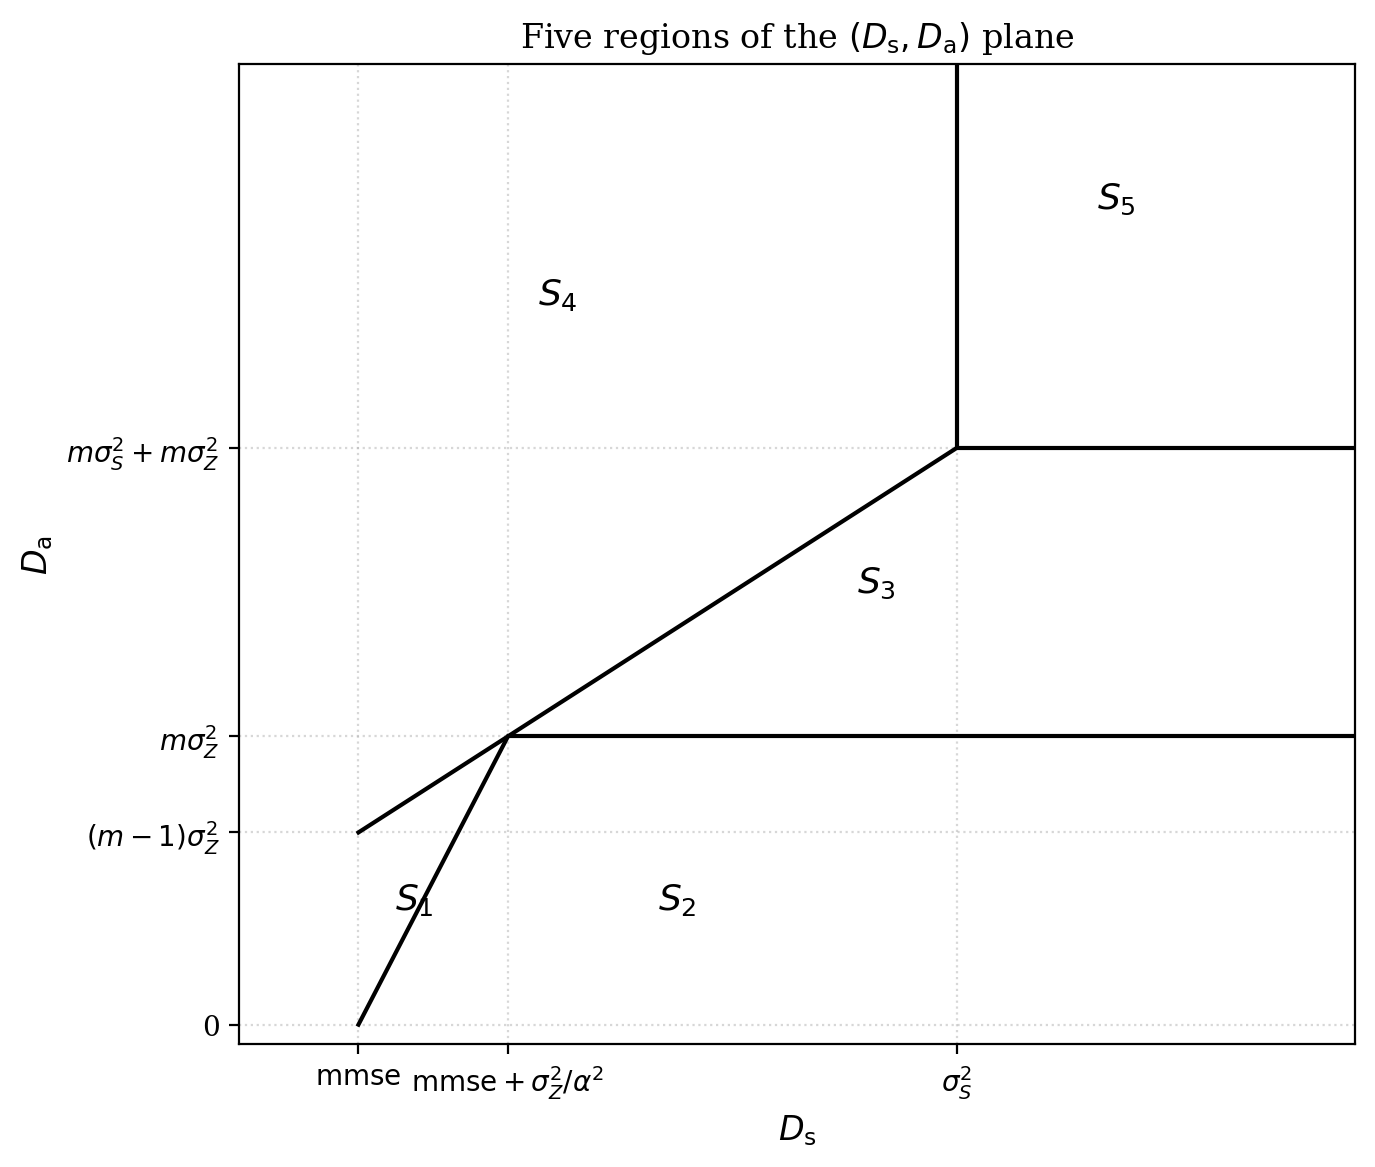
\includegraphics[width=\columnwidth]{../rd-semantic-repro/figures/fig2_five_regions.png}}
\caption{Illustration of the five regions of the $(D_s, D_a)$ plane for the jointly Gaussian vector model ($m=3$, $\sigma_S^2=1$, $\sigma_Z^2=1$).}
\label{fig:fig2}
\end{figure}

Fig.~\ref{fig:fig3} displays the 3D surface and contour plot of $R(D_s, D_a)$. The surface exhibits distinct behaviors: in region $S_5$, zero rate is achievable when both distortion constraints are sufficiently loose; in regions $S_1$ through $S_4$, the rate increases as the constraints tighten, with different functional forms in each region.

\begin{figure}[htbp]
\centerline{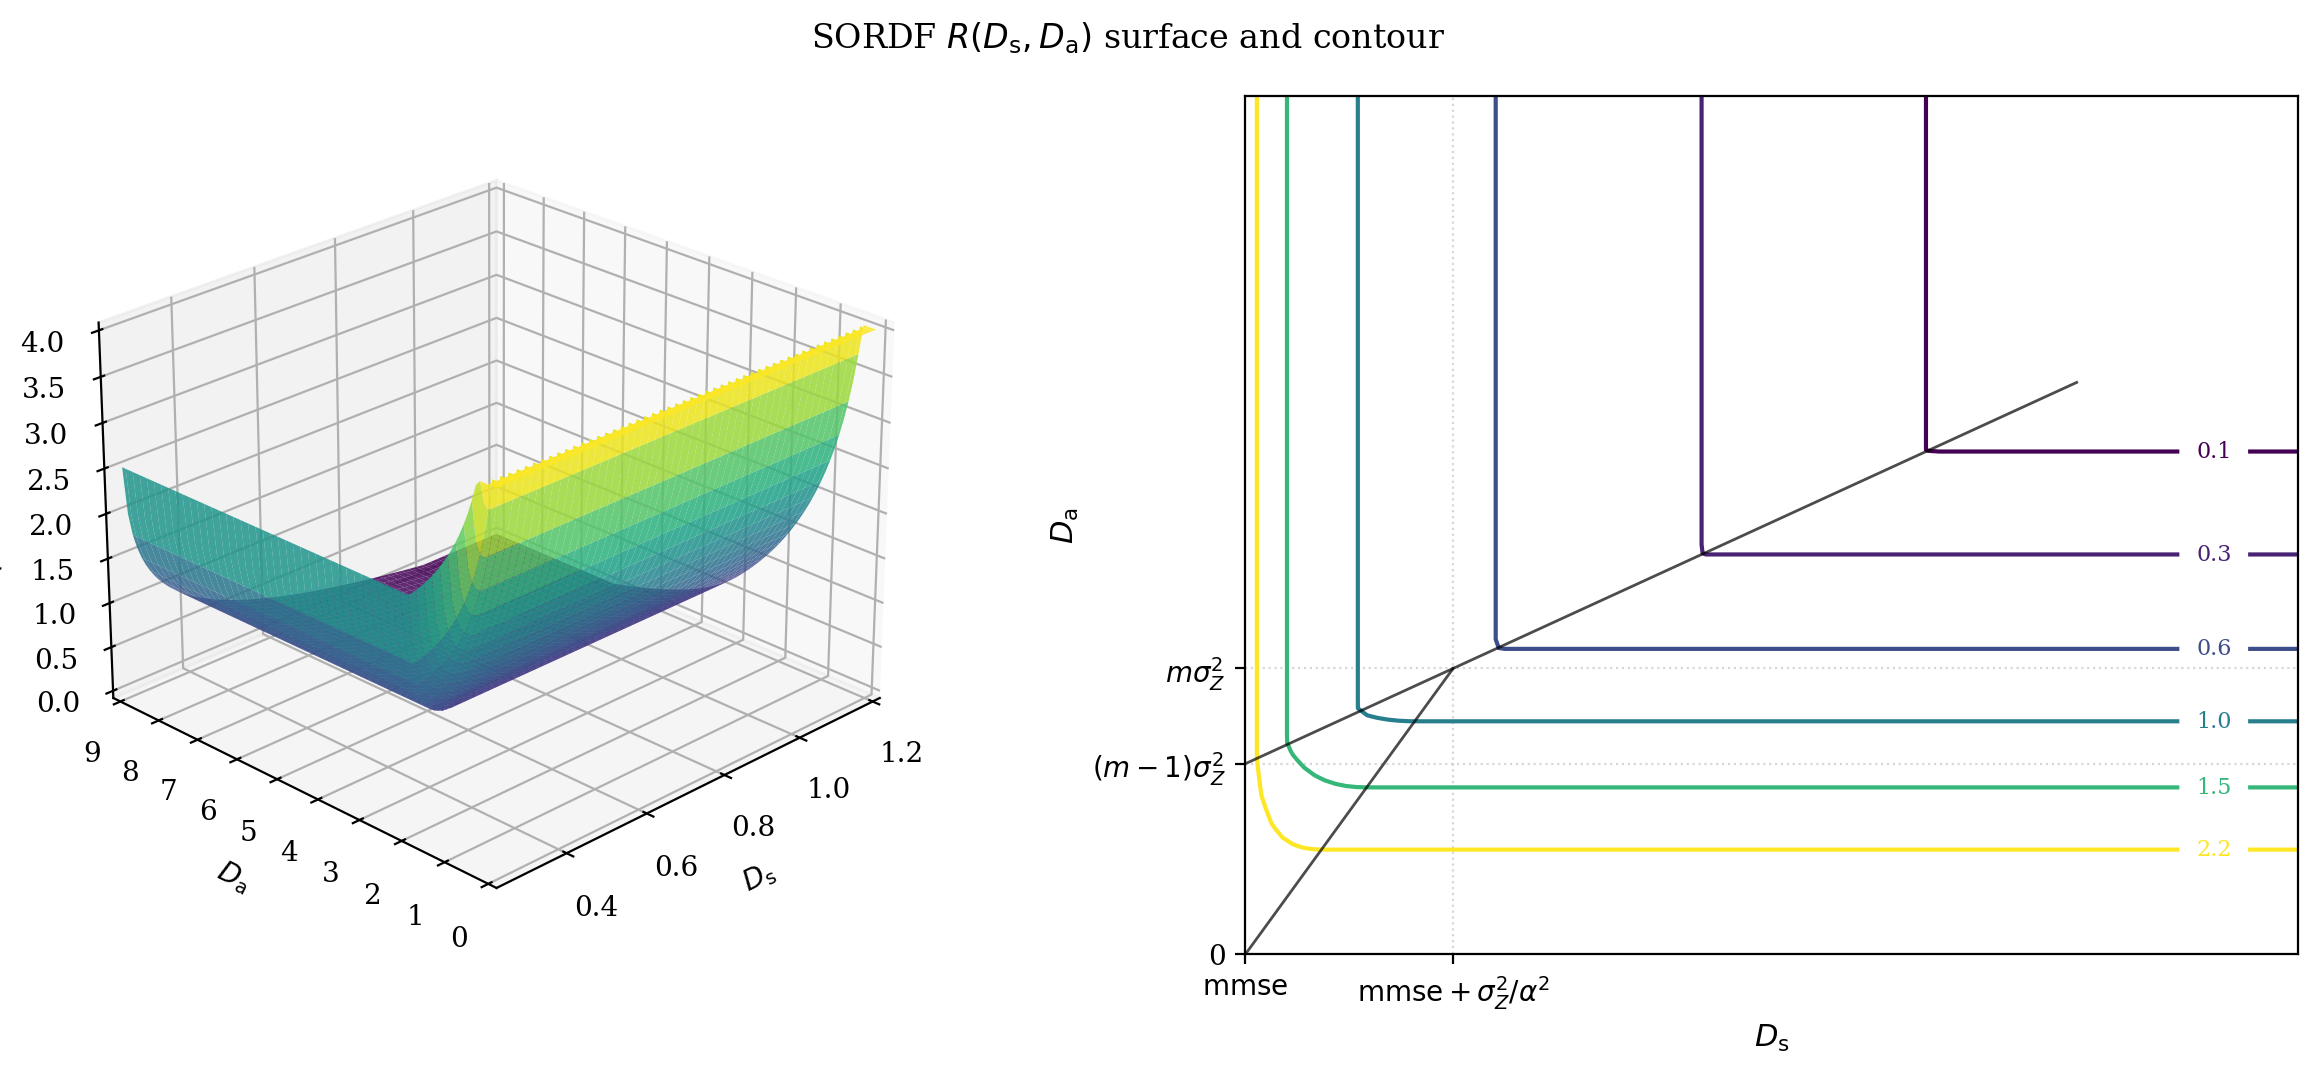
\includegraphics[width=\columnwidth]{../rd-semantic-repro/figures/fig3_sordf_3d_contour.png}}
\caption{The SORDF $R(D_s, D_a)$ as a 3D surface (left) and its contour plot (right).}
\label{fig:fig3}
\end{figure}

\section{Case 2: Binary Classification with Soft Decision}

\subsection{Problem Setup}

In the binary classification case, the semantic state $S$ is a binary label with uniform prior, and the observation $X$ is conditionally Gaussian:
\begin{equation}
S \sim \text{Bernoulli}(1/2), \quad
X|S=0 \sim \mathcal{N}(A, \sigma^2), \quad
X|S=1 \sim \mathcal{N}(-A, \sigma^2).
\end{equation}
Semantic distortion is Hamming distance (classification error rate), and we first consider unconstrained appearance ($D_a = \infty$).

\subsection{Soft vs. Hard Decision}

The Bayes optimal classification error rate is $P_e^* = Q(A/\sigma)$, where $Q(\cdot)$ is the Gaussian tail function. A naive approach would first perform hard Bayesian classification on $X$ and then compress the binary decision. However, Proposition 5 of \cite{liu2021rate} shows this is suboptimal.

The optimal scheme uses a \textbf{soft decision} function:
\begin{equation}
g(x) = \left[1 + \exp\left(\lambda \frac{1 - e^{-2Ax/\sigma^2}}{1 + e^{-2Ax/\sigma^2}}\right)\right]^{-1},
\end{equation}
where $\lambda < 0$ is a Lagrange multiplier chosen to satisfy the distortion constraint. The optimal rate is:
\begin{equation}
R(D_s, \infty) = 1 - \frac{1}{2}\int_{-\infty}^{\infty} [N^+(x) + N^-(x)]\, h_2(g(x))\, dx,
\end{equation}
where $N^+(x)$ and $N^-(x)$ are the conditional Gaussian densities, and $h_2(\cdot)$ is the binary entropy function.

\subsection{Numerical Results}

Fig.~\ref{fig:fig4} presents the key results. The left panel shows the soft decision function $g(x)$ under four different semantic distortion targets. As $D_s$ approaches the Bayes error $Q(A/\sigma) \approx 0.1587$, $g(x)$ approaches a hard step function. As $D_s \to 0.5$, $g(x)$ flattens to $0.5$, indicating no information about $S$ is preserved.

The right panel compares the rate-distortion curves of the optimal soft decision scheme versus the naive hard-decision-then-compress scheme. The gap between the two curves quantifies the benefit of joint optimization: the soft decision approach achieves strictly lower rates for the same semantic distortion, except at the extreme point $D_s = Q(A/\sigma)$ where both coincide.

\begin{figure}[htbp]
\centerline{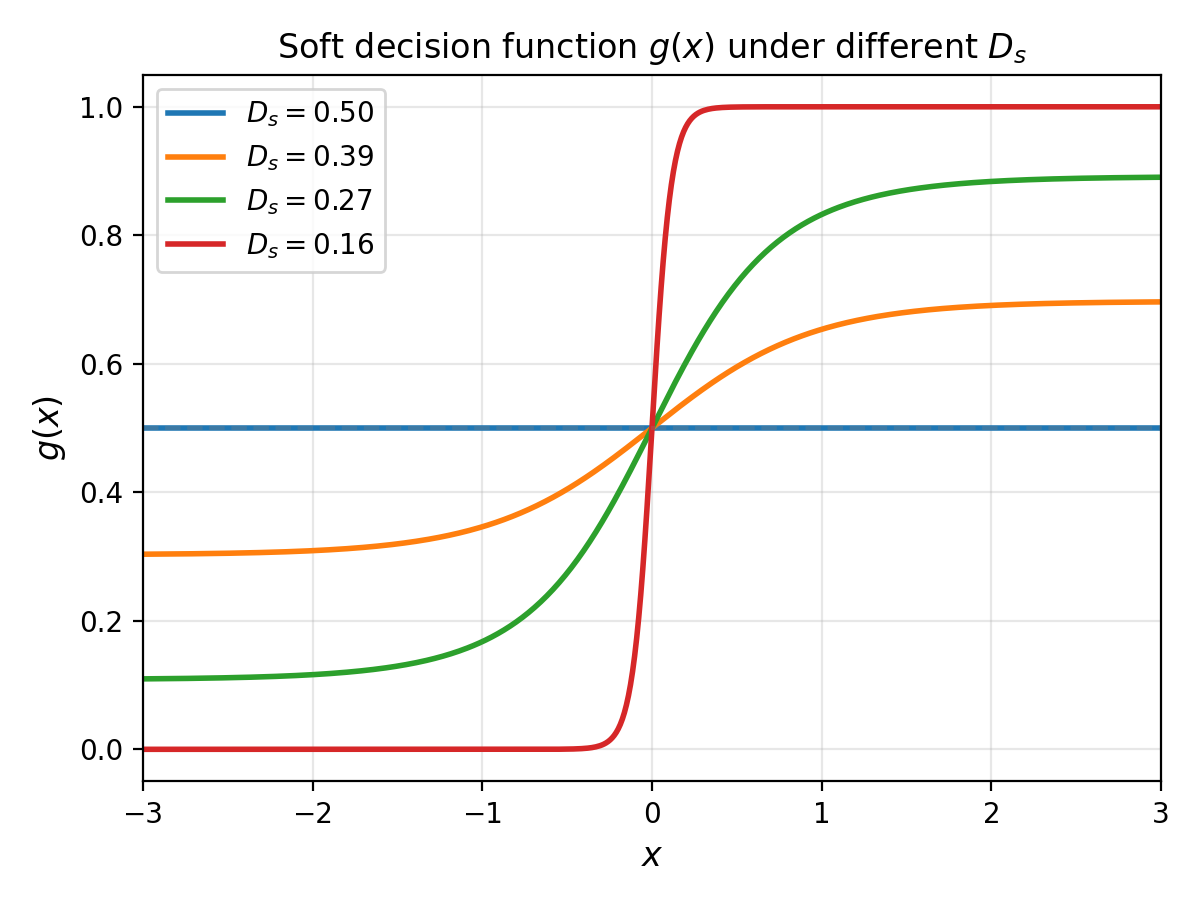
\includegraphics[width=\columnwidth]{../rd-semantic-repro/figures/fig4_left_gx.png}}
\caption{Left: Soft decision function $g(x)$ under different $D_s$. Right: Rate-distortion comparison between optimal soft decision and naive hard decision schemes ($A=1$, $\sigma=1$).}
\label{fig:fig4}
\end{figure}

\begin{figure}[htbp]
\centerline{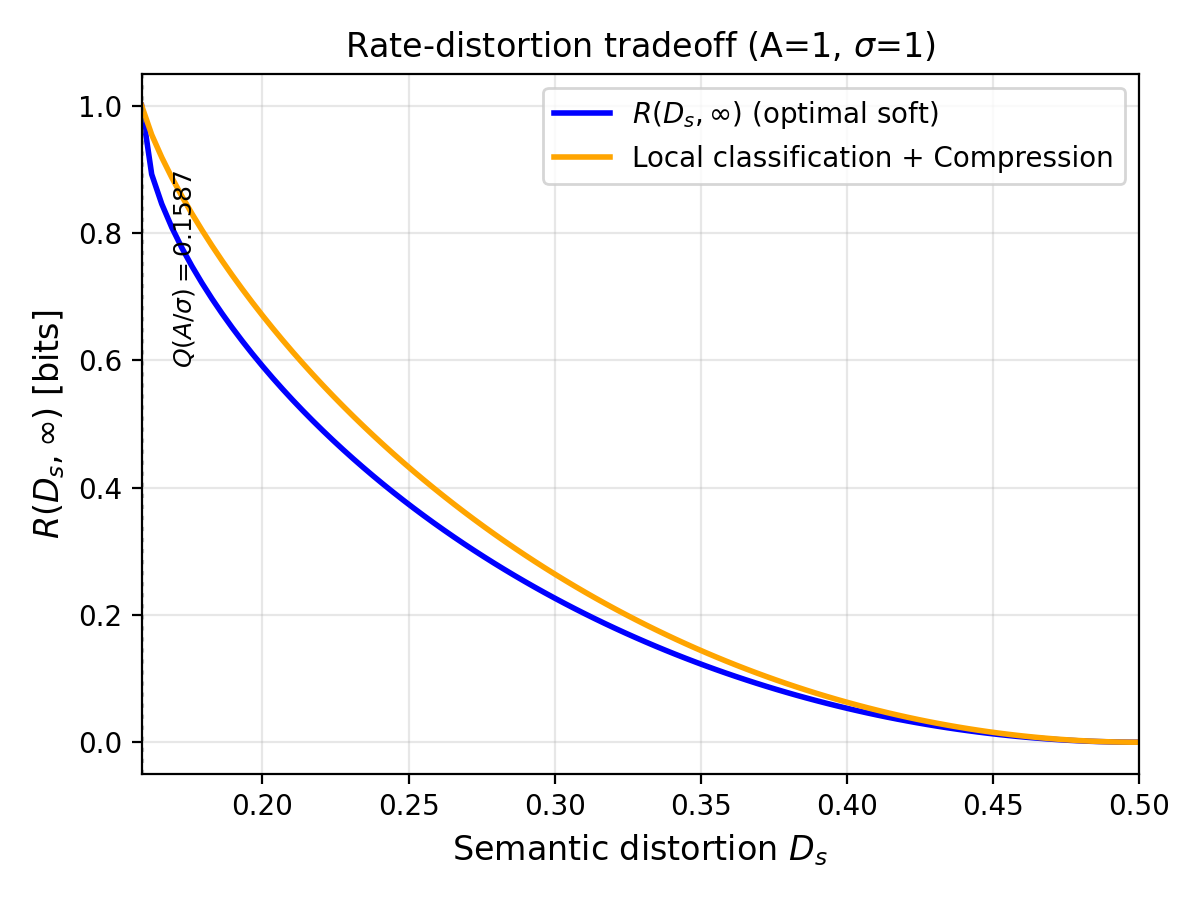
\includegraphics[width=\columnwidth]{../rd-semantic-repro/figures/fig4_right_rd.png}}
\caption{Rate-distortion tradeoff: optimal soft decision vs.\ naive hard-decision-then-compress.}
\label{fig:fig4b}
\end{figure}

\section{Case 3: Joint Rate-Distortion with Double Constraints}

\subsection{Achievable Upper Bound}

When both semantic and appearance constraints are active, Proposition 6 of \cite{liu2021rate} provides an achievable upper bound via a two-stage coding scheme. Stage 1 encodes the semantic information using the soft decision framework, producing an intermediate representation with semantic distortion $D \leq D_s$. Stage 2 encodes the appearance residual conditioned on the semantic reconstruction.

The achievable rate is:
\begin{equation}
R_{\text{ach}}(D_s, D_a) = \min_{D \in [Q(A/\sigma), D_s]} \left[ R(D, \infty) + \frac{1}{2}\log_2^+\frac{\eta(D)}{D_a} \right],
\end{equation}
where $\eta(D) = \mathbb{E}[(X - \gamma(D))^2 \cdot g(X)]$ is the residual variance after semantic encoding, and $\gamma(D) = \mathbb{E}[X \cdot g(X)]$ is the conditional mean.

\subsection{Numerical Results}

Fig.~\ref{fig:fig5} shows the achievable upper bound curves for three different semantic distortion targets ($D_s = 0.50, 0.30, 0.10$) with $A^2/\sigma^2 = 10$. Two baselines are also plotted: direct encoding of $X$ (ignoring semantics), and the ideal case where $S$ is known exactly.

As $D_s$ decreases (stricter semantic requirement), the rate increases for all appearance distortion levels. When $D_a$ is large (loose appearance constraint), the rate approaches $R(D_s, \infty)$. When $D_a$ becomes very small, the rate diverges as the system must spend additional bits to satisfy the tight appearance constraint.

\begin{figure}[htbp]
\centerline{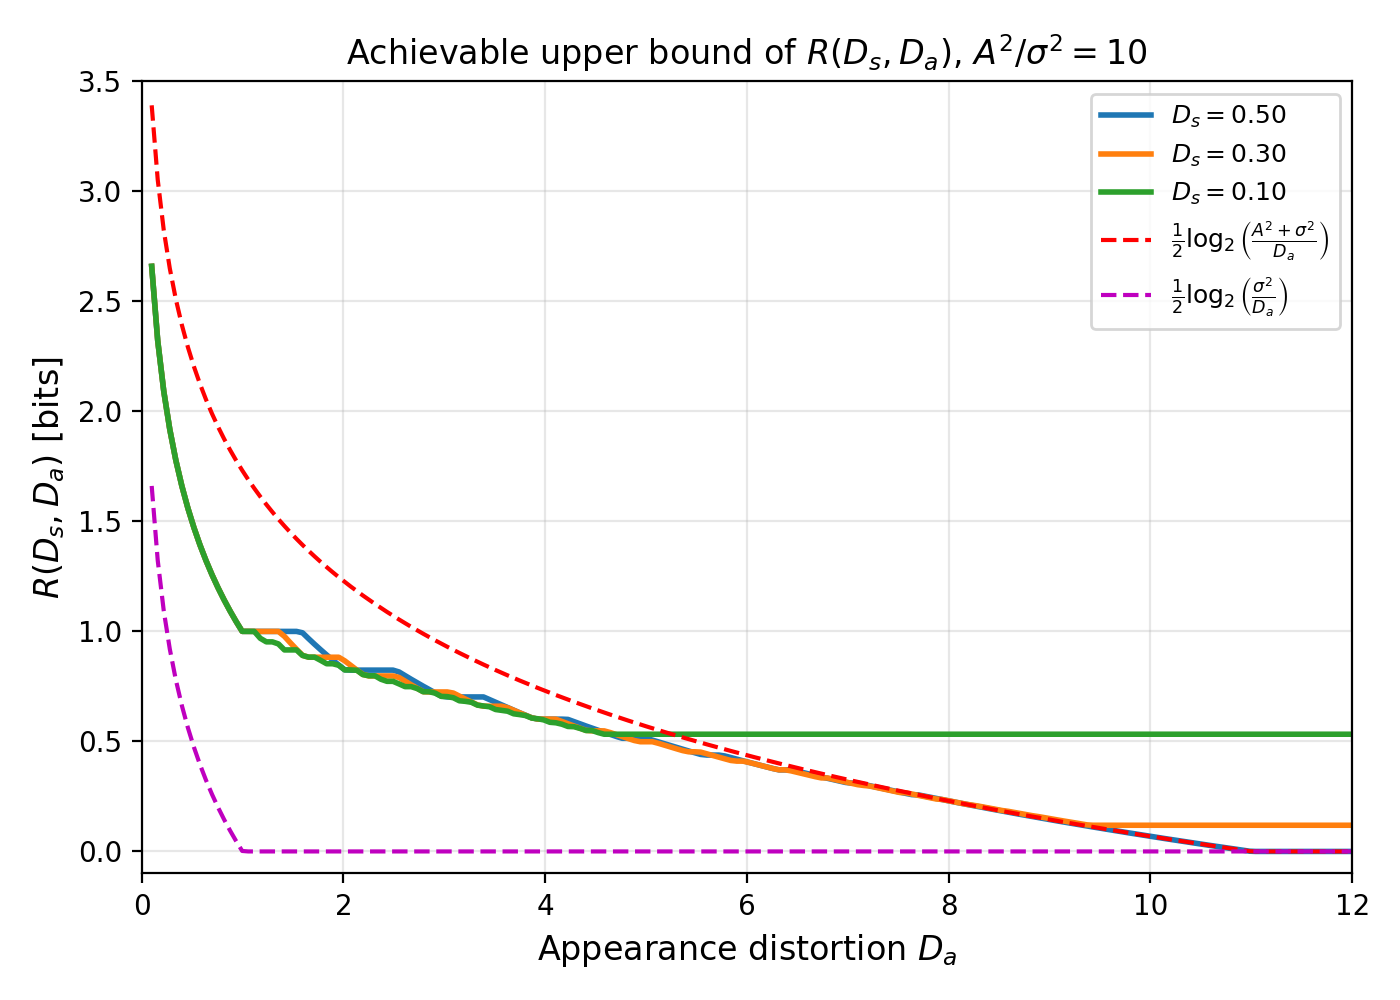
\includegraphics[width=\columnwidth]{../rd-semantic-repro/figures/fig5_joint_rd.png}}
\caption{Achievable upper bound of $R(D_s, D_a)$ for $A^2/\sigma^2 = 10$, under three semantic distortion targets.}
\label{fig:fig5}
\end{figure}

\section{Extension: RDPC Framework on MNIST}

\subsection{Motivation and Formulation}

The original SORDF framework uses pixel-wise MSE as the appearance distortion, which is known to produce blurry reconstructions. Inspired by recent work on perception-constrained compression \cite{blau2019rethinking}, we introduce a third constraint---perceptual quality---into the framework.

We formulate the \textbf{Rate-Distortion-Perception-Classification (RDPC)} problem:
\begin{equation}
R(D, P, C) = \min_{p(\hat{x}|x)} I(X; \hat{X})
\end{equation}
subject to:
\begin{align}
\mathbb{E}[\Delta(X, \hat{X})] &\leq D \quad \text{(Reconstruction)} \\
d_{\text{W}}(p_X, p_{\hat{X}}) &\leq P \quad \text{(Perception)} \\
H(S \mid \hat{X}) &\leq C \quad \text{(Classification)}
\end{align}
where $d_{\text{W}}$ is the Wasserstein distance and $H(S \mid \hat{X})$ bounds the classification uncertainty.

\subsection{Deep Learning Architecture}

We implement the RDPC framework using a deep autoencoder with three learning objectives, as shown in Fig.~\ref{fig:arch}:
\begin{itemize}
    \item \textbf{Encoder}: CNN mapping $X \in \mathbb{R}^{28\times28}$ to latent $Z \in \mathbb{R}^k$ (rate controlled by latent dimension $k$);
    \item \textbf{Decoder}: Transposed CNN reconstructing $\hat{X}$ from $Z$;
    \item \textbf{Discriminator}: WGAN-GP critic enforcing the perception constraint via gradient penalty;
    \item \textbf{Classifier}: Pre-trained frozen CNN providing semantic supervision on $\hat{X}$.
\end{itemize}

The joint training loss is:
\begin{equation}
\mathcal{L} = \lambda_d \cdot \text{MSE}(x, \hat{x}) - \lambda_p \cdot D(\hat{x}) + \lambda_c \cdot \text{CE}(s, \hat{s}),
\end{equation}
where $D(\hat{x})$ is the discriminator score (higher = more realistic), and CE is cross-entropy loss.

\subsection{Experimental Results}

We conducted a sweep over latent dimensions $k \in \{4, 8, 16, 32, 64\}$ and Lagrange multipliers $\lambda_p \in \{0.01, 0.1, 1.0\}$, $\lambda_c \in \{0.1, 1.0, 10.0\}$, with $\lambda_d = 1.0$ fixed. Table~\ref{tab:sweep} presents representative results.

\begin{table}[htbp]
\caption{Representative RDPC sweep results on MNIST (20 epochs).}
\begin{center}
\begin{tabular}{cccccc}
\toprule
$k$ & $\lambda_p$ & $\lambda_c$ & Rate (bits) & MSE & Acc (\%) \\
\midrule
4  & 0.01 & 0.1  & 9.50  & 31.52 & 98.01 \\
4  & 1.0  & 10.0 & 10.64 & 54.90 & 97.85 \\
16 & 0.01 & 1.0  & 41.67 & 33.44 & 98.98 \\
16 & 0.1  & 1.0  & 42.22 & 24.27 & 98.24 \\
16 & 1.0  & 10.0 & 41.64 & 36.61 & 97.76 \\
32 & 0.1  & 1.0  & 81.25 & 19.41 & 98.45 \\
64 & 0.1  & 0.1  & 180.0 & 12.21 & 98.15 \\
\bottomrule
\end{tabular}
\label{tab:sweep}
\end{center}
\end{table}

Several observations emerge:
\begin{enumerate}
    \item \textbf{Rate-dimension relationship}: The estimated rate scales approximately linearly with the latent dimension $k$, consistent with the Gaussian entropy upper bound $R \approx \frac{1}{2}\sum_i \log(1 + \sigma_i^2)$.
    \item \textbf{Perception-distortion tradeoff}: Increasing $\lambda_p$ (stronger perception constraint) generally increases MSE. At $k=16$, raising $\lambda_p$ from 0.01 to 1.0 while fixing $\lambda_c=10.0$ changes MSE from 86.31 to 36.61 (with different $\lambda_c$, the trend is modulated by the classification term).
    \item \textbf{Classification robustness}: The classification accuracy remains above 97\% across most configurations, demonstrating that semantic information can be preserved even under tight rate and perception constraints. The lowest accuracy (87.22\%) occurs at $(k=4, \lambda_p=1.0, \lambda_c=0.1)$, where strong perception pressure dominates at very low rate.
    \item \textbf{Three-way tradeoff}: At fixed rate (e.g., $k=16$), varying $(\lambda_p, \lambda_c)$ traces a 2D tradeoff surface. Higher $\lambda_p$ improves perceptual quality at the cost of MSE; higher $\lambda_c$ improves classification at the cost of both MSE and perceptual quality.
\end{enumerate}

\section{Implementation and Testing Methodology}

All theoretical computations are implemented in Python using NumPy, SciPy, and Matplotlib. The SORDF computations involve:
\begin{itemize}
    \item Numerical integration via adaptive quadrature (\texttt{scipy.integrate.quad});
    \item Root-finding for the Lagrange multiplier $\lambda$ via Brent's method (\texttt{scipy.optimize.brentq});
    \item Gaussian Q-function and binary entropy function implementations.
\end{itemize}

The codebase follows a test-driven development approach. Each theorem-level claim from the paper is encoded as a boundary-condition test:
\begin{itemize}
    \item $D_s < Q(A/\sigma)$ is infeasible (raises \texttt{ValueError});
    \item At $D_s = Q(A/\sigma)$, the rate equals 1 bit;
    \item At $D_s = 0.5$, the rate is zero;
    \item Better class separation (larger $A/\sigma$) reduces the minimum achievable $D_s$;
    \item The rate function is monotone non-increasing in $D_s$.
\end{itemize}

The deep learning pipeline uses PyTorch with a WGAN-GP training regime. The discriminator is updated $n_{\text{critic}} = 5$ times per generator update, with gradient penalty weight $\lambda_{\text{gp}} = 10$. The classifier is pre-trained for 5 epochs on clean MNIST images and frozen during RDPC training.

\section{Conclusion}

This project provides a comprehensive reproduction and extension of the rate-distortion framework for semantic information. On the theoretical side, we numerically validated the SORDF across three canonical cases: the vector Gaussian model with its five-region phase diagram, the binary classification model revealing the optimality of soft decision over hard Bayesian classification, and the joint constraint setting with an achievable two-stage coding bound.

On the practical side, we extended the framework to include a perception constraint via WGAN-GP, formulating the RDPC problem. Deep learning experiments on MNIST demonstrate the feasibility of simultaneously optimizing for reconstruction quality, perceptual realism, and classification accuracy, and reveal the rich tradeoff surfaces among these three objectives under rate constraints.

Future work includes developing neural estimators for the SORDF that can operate on high-dimensional data without closed-form solutions, extending the RDPC framework to more complex datasets (e.g., CIFAR-10, ImageNet), and investigating whether the soft-decision optimality result generalizes to deep learning-based semantic communication systems.

\begin{thebibliography}{00}
\bibitem{liu2021rate} J. Liu, W. Zhang, and H. V. Poor, ``A rate-distortion framework for characterizing semantic information,'' in \textit{Proc. IEEE Int. Symp. Inf. Theory (ISIT)}, 2021.
\bibitem{blau2019rethinking} Y. Blau and T. Michaeli, ``Rethinking lossy compression: The rate-distortion-perception tradeoff,'' in \textit{Proc. Int. Conf. Mach. Learn. (ICML)}, 2019.
\bibitem{cover2006elements} T. M. Cover and J. A. Thomas, \textit{Elements of Information Theory}, 2nd ed. Wiley, 2006.
\bibitem{shannon1959coding} C. E. Shannon, ``Coding theorems for a discrete source with a fidelity criterion,'' \textit{IRE Nat. Conv. Rec.}, vol. 7, pp. 142--163, 1959.
\end{thebibliography}

\end{document}
